% Gradient Info

\tikzset {_audied9e7/.code = {\pgfsetadditionalshadetransform{ \pgftransformshift{\pgfpoint{0 bp } { 45 bp }  }  \pgftransformscale{3 }  }}}
\pgfdeclareradialshading{_l1th8ezcg}{\pgfpoint{0bp}{-16bp}}{rgb(0bp)=(0.91,0.88,0.88);
	rgb(0bp)=(0.91,0.88,0.88);
	rgb(12.678571428571427bp)=(0.74,0.73,0.73);
	rgb(25bp)=(0.74,0.73,0.73);
	rgb(400bp)=(0.74,0.73,0.73)}

% Gradient Info

\tikzset {_zw799en1h/.code = {\pgfsetadditionalshadetransform{ \pgftransformshift{\pgfpoint{0 bp } { 0 bp }  }  \pgftransformscale{3 }  }}}
\pgfdeclareradialshading{_7fov45wgl}{\pgfpoint{0bp}{0bp}}{rgb(0bp)=(0.9,0.89,0.89);
	rgb(0bp)=(0.9,0.89,0.89);
	rgb(14.196428571428571bp)=(0.8,0.77,0.77);
	rgb(25bp)=(0.74,0.72,0.72);
	rgb(400bp)=(0.74,0.72,0.72)}

% Gradient Info

\tikzset {_ma7ryb15k/.code = {\pgfsetadditionalshadetransform{ \pgftransformshift{\pgfpoint{116.1 bp } { -141.9 bp }  }  \pgftransformscale{1.72 }  }}}
\pgfdeclareradialshading{_l971no8s8}{\pgfpoint{-72bp}{88bp}}{rgb(0bp)=(0.9,0.89,0.89);
	rgb(0bp)=(0.9,0.89,0.89);
	rgb(4.196428571428571bp)=(0.9,0.89,0.89);
	rgb(8.303571428571429bp)=(0.9,0.89,0.89);
	rgb(12.857142857142856bp)=(0.93,0.89,0.89);
	rgb(25bp)=(0.67,0.66,0.66);
	rgb(400bp)=(0.67,0.66,0.66)}

% Gradient Info

\tikzset {_f6tcg567o/.code = {\pgfsetadditionalshadetransform{ \pgftransformshift{\pgfpoint{0 bp } { 0 bp }  }  \pgftransformscale{1.38 }  }}}
\pgfdeclareradialshading{_u0fs4tjoa}{\pgfpoint{0bp}{0bp}}{rgb(0bp)=(0.85,0.85,0.85);
	rgb(0bp)=(0.85,0.85,0.85);
	rgb(11.875bp)=(0.83,0.82,0.82);
	rgb(25bp)=(0.69,0.68,0.68);
	rgb(400bp)=(0.69,0.68,0.68)}

% Gradient Info

\tikzset {_kvu3t6wn8/.code = {\pgfsetadditionalshadetransform{ \pgftransformshift{\pgfpoint{0 bp } { 0 bp }  }  \pgftransformscale{3 }  }}}
\pgfdeclareradialshading{_ifkxbtcrd}{\pgfpoint{0bp}{0bp}}{rgb(0bp)=(0.9,0.89,0.89);
	rgb(0bp)=(0.9,0.89,0.89);
	rgb(14.196428571428571bp)=(0.8,0.77,0.77);
	rgb(25bp)=(0.74,0.72,0.72);
	rgb(400bp)=(0.74,0.72,0.72)}

% Gradient Info

\tikzset {_relekxdrh/.code = {\pgfsetadditionalshadetransform{ \pgftransformshift{\pgfpoint{0 bp } { 0 bp }  }  \pgftransformscale{1.38 }  }}}
\pgfdeclareradialshading{_i9ec3u4oc}{\pgfpoint{0bp}{0bp}}{rgb(0bp)=(0.85,0.85,0.85);
	rgb(0bp)=(0.85,0.85,0.85);
	rgb(11.875bp)=(0.83,0.82,0.82);
	rgb(25bp)=(0.69,0.68,0.68);
	rgb(400bp)=(0.69,0.68,0.68)}
\tikzset{every picture/.style={line width=0.75pt}} %set default line width to 0.75pt        

\begin{figure}[H]
	\centering
	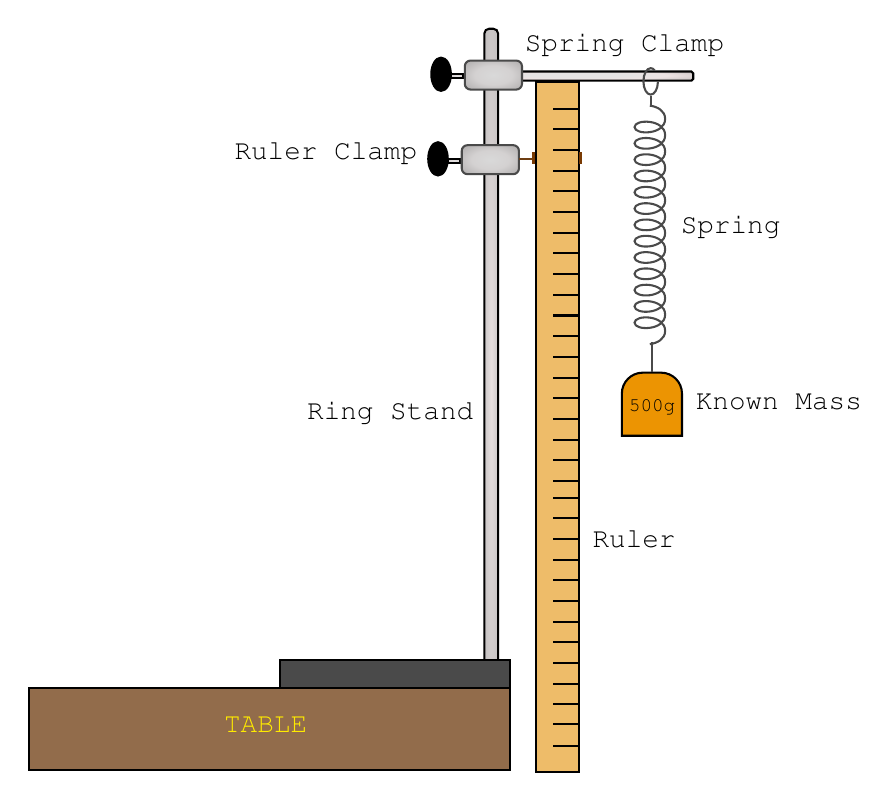
\begin{tikzpicture}[x=0.75pt,y=0.75pt,yscale=-1,xscale=1]

		%uncomment if require: \path (0,480); %set diagram left start at 0, and has height of 480

		%Shape: Rectangle [id:dp661407400810794] 
		\draw  [fill={rgb, 255:red, 146; green, 108; blue, 75 }  ,fill opacity=1 ] (137.34,380.7) -- (369.11,380.7) -- (369.11,419.99) -- (137.34,419.99) -- cycle ;
		%Rounded Rect [id:dp14042717508972213] 
		\path  [shading=_l1th8ezcg,_audied9e7] (356.84,65.35) .. controls (356.84,64.05) and (357.89,63) .. (359.19,63) -- (361.15,63) .. controls (362.45,63) and (363.5,64.05) .. (363.5,65.35) -- (363.5,369.65) .. controls (363.5,370.95) and (362.45,372) .. (361.15,372) -- (359.19,372) .. controls (357.89,372) and (356.84,370.95) .. (356.84,369.65) -- cycle ; % for fading 
		\draw   (356.84,65.35) .. controls (356.84,64.05) and (357.89,63) .. (359.19,63) -- (361.15,63) .. controls (362.45,63) and (363.5,64.05) .. (363.5,65.35) -- (363.5,369.65) .. controls (363.5,370.95) and (362.45,372) .. (361.15,372) -- (359.19,372) .. controls (357.89,372) and (356.84,370.95) .. (356.84,369.65) -- cycle ; % for border 

		%Shape: Spring [id:dp16658294194788303] 
		\draw  [color={rgb, 255:red, 74; green, 74; blue, 74 }  ,draw opacity=1 ][line width=0.75]  (436.59,100.06) .. controls (440.27,100.55) and (443.96,102.52) .. (443.96,106.44) .. controls (443.96,114.3) and (429.22,114.3) .. (429.22,110.37) .. controls (429.22,106.44) and (443.96,106.44) .. (443.96,114.3) .. controls (443.96,122.16) and (429.22,122.16) .. (429.22,118.23) .. controls (429.22,114.3) and (443.96,114.3) .. (443.96,122.16) .. controls (443.96,130.01) and (429.22,130.01) .. (429.22,126.09) .. controls (429.22,122.16) and (443.96,122.16) .. (443.96,130.01) .. controls (443.96,137.87) and (429.22,137.87) .. (429.22,133.94) .. controls (429.22,130.01) and (443.96,130.01) .. (443.96,137.87) .. controls (443.96,145.73) and (429.22,145.73) .. (429.22,141.8) .. controls (429.22,137.87) and (443.96,137.87) .. (443.96,145.73) .. controls (443.96,153.58) and (429.22,153.58) .. (429.22,149.66) .. controls (429.22,145.73) and (443.96,145.73) .. (443.96,153.58) .. controls (443.96,161.44) and (429.22,161.44) .. (429.22,157.51) .. controls (429.22,153.58) and (443.96,153.58) .. (443.96,161.44) .. controls (443.96,169.3) and (429.22,169.3) .. (429.22,165.37) .. controls (429.22,161.44) and (443.96,161.44) .. (443.96,169.3) .. controls (443.96,177.15) and (429.22,177.15) .. (429.22,173.23) .. controls (429.22,169.3) and (443.96,169.3) .. (443.96,177.15) .. controls (443.96,185.01) and (429.22,185.01) .. (429.22,181.08) .. controls (429.22,177.15) and (443.96,177.15) .. (443.96,185.01) .. controls (443.96,192.87) and (429.22,192.87) .. (429.22,188.94) .. controls (429.22,185.01) and (443.96,185.01) .. (443.96,192.87) .. controls (443.96,200.72) and (429.22,200.72) .. (429.22,196.8) .. controls (429.22,192.87) and (443.96,192.87) .. (443.96,200.72) .. controls (443.96,208.58) and (429.22,208.58) .. (429.22,204.65) .. controls (429.22,200.72) and (443.96,200.72) .. (443.96,208.58) .. controls (443.96,212.51) and (440.27,214.47) .. (436.59,214.96) ;
		%Shape: Rectangle [id:dp22739131790719957] 
		\path  [shading=_7fov45wgl,_zw799en1h] (340.72,84.94) -- (346.77,84.94) -- (346.77,86.73) -- (340.72,86.73) -- cycle ; % for fading 
		\draw  [color={rgb, 255:red, 0; green, 0; blue, 0 }  ,draw opacity=1 ] (340.72,84.94) -- (346.77,84.94) -- (346.77,86.73) -- (340.72,86.73) -- cycle ; % for border 

		%Rounded Rect [id:dp8164684948783012] 
		\path  [shading=_l971no8s8,_ma7ryb15k] (365.18,84.51) .. controls (365.18,84.02) and (365.58,83.62) .. (366.07,83.62) -- (456.62,83.62) .. controls (457.1,83.62) and (457.5,84.02) .. (457.5,84.51) -- (457.5,87.16) .. controls (457.5,87.65) and (457.1,88.04) .. (456.62,88.04) -- (366.07,88.04) .. controls (365.58,88.04) and (365.18,87.65) .. (365.18,87.16) -- cycle ; % for fading 
		\draw   (365.18,84.51) .. controls (365.18,84.02) and (365.58,83.62) .. (366.07,83.62) -- (456.62,83.62) .. controls (457.1,83.62) and (457.5,84.02) .. (457.5,84.51) -- (457.5,87.16) .. controls (457.5,87.65) and (457.1,88.04) .. (456.62,88.04) -- (366.07,88.04) .. controls (365.58,88.04) and (365.18,87.65) .. (365.18,87.16) -- cycle ; % for border 

		%Rounded Same Side Corner Rect [id:dp3337767177690609] 
		\draw  [fill={rgb, 255:red, 236; green, 148; blue, 2 }  ,fill opacity=1 ] (423.11,238.8) .. controls (423.11,233.23) and (427.62,228.71) .. (433.19,228.71) -- (441.99,228.71) .. controls (447.56,228.71) and (452.08,233.23) .. (452.08,238.8) -- (452.08,259.09) .. controls (452.08,259.09) and (452.08,259.09) .. (452.08,259.09) -- (423.11,259.09) .. controls (423.11,259.09) and (423.11,259.09) .. (423.11,259.09) -- cycle ;
		%Straight Lines [id:da9036000547278182] 
		\draw [color={rgb, 255:red, 74; green, 74; blue, 74 }  ,draw opacity=1 ]   (437.57,228.22) -- (437.57,213.98) ;
		%Rounded Rect [id:dp8364710468830279] 
		\path  [shading=_u0fs4tjoa,_f6tcg567o] (347.44,81.14) .. controls (347.44,79.59) and (348.69,78.34) .. (350.24,78.34) -- (372.21,78.34) .. controls (373.75,78.34) and (375.01,79.59) .. (375.01,81.14) -- (375.01,89.53) .. controls (375.01,91.07) and (373.75,92.32) .. (372.21,92.32) -- (350.24,92.32) .. controls (348.69,92.32) and (347.44,91.07) .. (347.44,89.53) -- cycle ; % for fading 
		\draw  [color={rgb, 255:red, 74; green, 74; blue, 74 }  ,draw opacity=1 ] (347.44,81.14) .. controls (347.44,79.59) and (348.69,78.34) .. (350.24,78.34) -- (372.21,78.34) .. controls (373.75,78.34) and (375.01,79.59) .. (375.01,81.14) -- (375.01,89.53) .. controls (375.01,91.07) and (373.75,92.32) .. (372.21,92.32) -- (350.24,92.32) .. controls (348.69,92.32) and (347.44,91.07) .. (347.44,89.53) -- cycle ; % for border 

		%Shape: Ellipse [id:dp5179670735428143] 
		\draw  [fill={rgb, 255:red, 0; green, 0; blue, 0 }  ,fill opacity=1 ] (331.3,84.94) .. controls (331.3,80.52) and (333.41,76.93) .. (336.01,76.93) .. controls (338.61,76.93) and (340.72,80.52) .. (340.72,84.94) .. controls (340.72,89.37) and (338.61,92.95) .. (336.01,92.95) .. controls (333.41,92.95) and (331.3,89.37) .. (331.3,84.94) -- cycle ;
		%Shape: Rectangle [id:dp7277974618781018] 
		\path  [shading=_ifkxbtcrd,_kvu3t6wn8] (339.24,125.7) -- (345.29,125.7) -- (345.29,127.49) -- (339.24,127.49) -- cycle ; % for fading 
		\draw  [color={rgb, 255:red, 0; green, 0; blue, 0 }  ,draw opacity=1 ] (339.24,125.7) -- (345.29,125.7) -- (345.29,127.49) -- (339.24,127.49) -- cycle ; % for border 

		%Rounded Rect [id:dp9330549543329489] 
		\path  [shading=_i9ec3u4oc,_relekxdrh] (345.97,121.89) .. controls (345.97,120.35) and (347.22,119.1) .. (348.76,119.1) -- (370.74,119.1) .. controls (372.28,119.1) and (373.53,120.35) .. (373.53,121.89) -- (373.53,130.28) .. controls (373.53,131.83) and (372.28,133.08) .. (370.74,133.08) -- (348.76,133.08) .. controls (347.22,133.08) and (345.97,131.83) .. (345.97,130.28) -- cycle ; % for fading 
		\draw  [color={rgb, 255:red, 74; green, 74; blue, 74 }  ,draw opacity=1 ] (345.97,121.89) .. controls (345.97,120.35) and (347.22,119.1) .. (348.76,119.1) -- (370.74,119.1) .. controls (372.28,119.1) and (373.53,120.35) .. (373.53,121.89) -- (373.53,130.28) .. controls (373.53,131.83) and (372.28,133.08) .. (370.74,133.08) -- (348.76,133.08) .. controls (347.22,133.08) and (345.97,131.83) .. (345.97,130.28) -- cycle ; % for border 

		%Shape: Ellipse [id:dp27429498112957074] 
		\draw  [fill={rgb, 255:red, 0; green, 0; blue, 0 }  ,fill opacity=1 ] (329.83,125.7) .. controls (329.83,121.28) and (331.94,117.69) .. (334.54,117.69) .. controls (337.14,117.69) and (339.24,121.28) .. (339.24,125.7) .. controls (339.24,130.12) and (337.14,133.71) .. (334.54,133.71) .. controls (331.94,133.71) and (329.83,130.12) .. (329.83,125.7) -- cycle ;
		%Straight Lines [id:da6364752459654412] 
		\draw [color={rgb, 255:red, 110; green, 61; blue, 18 }  ,draw opacity=1 ][line width=0.75]    (373.53,125.85) -- (380.9,125.85) ;
		%Shape: Rectangle [id:dp879583802615739] 
		\draw  [color={rgb, 255:red, 121; green, 58; blue, 3 }  ,draw opacity=1 ][fill={rgb, 255:red, 97; green, 47; blue, 4 }  ,fill opacity=1 ] (380.41,122.91) -- (380.9,122.91) -- (380.9,127.82) -- (380.41,127.82) -- cycle ;
		%Shape: Rectangle [id:dp2590872105368831] 
		\draw  [color={rgb, 255:red, 0; green, 0; blue, 0 }  ,draw opacity=1 ][fill={rgb, 255:red, 238; green, 188; blue, 105 }  ,fill opacity=1 ][line width=0.75]  (402.49,420.97) -- (381.86,420.97) -- (381.86,88.53) -- (402.49,88.53) -- cycle ;
		%Straight Lines [id:da4342154910571179] 
		\draw    (402.49,408.51) -- (389.72,408.51) ;
		%Straight Lines [id:da8960085846992045] 
		\draw    (402.49,398.04) -- (389.72,398.04) ;
		%Straight Lines [id:da29417082715176046] 
		\draw    (402.49,388.57) -- (389.72,388.57) ;
		%Straight Lines [id:da7043382052247802] 
		\draw    (402.49,378.6) -- (389.72,378.6) ;
		%Straight Lines [id:da14461348672257412] 
		\draw    (402.49,368.64) -- (389.72,368.64) ;
		%Straight Lines [id:da8812764216308848] 
		\draw    (402.49,358.67) -- (389.72,358.67) ;
		%Straight Lines [id:da46113320559838833] 
		\draw    (402.49,348.7) -- (389.72,348.7) ;
		%Straight Lines [id:da06870609801527894] 
		\draw    (402.49,338.73) -- (389.72,338.73) ;
		%Straight Lines [id:da6491635747766802] 
		\draw    (402.49,328.76) -- (389.72,328.76) ;
		%Straight Lines [id:da6541158039132522] 
		\draw    (402.49,318.8) -- (389.72,318.8) ;
		%Straight Lines [id:da8229925427369018] 
		\draw    (402.49,308.83) -- (389.72,308.83) ;
		%Straight Lines [id:da9289832823167388] 
		\draw    (402.49,298.86) -- (389.72,298.86) ;
		%Straight Lines [id:da1480662946592668] 
		\draw    (402.49,288.89) -- (389.72,288.89) ;
		%Straight Lines [id:da8076788219370534] 
		\draw    (402.49,280.92) -- (389.72,280.92) ;
		%Straight Lines [id:da7862953107859727] 
		\draw    (402.49,270.95) -- (389.72,270.95) ;
		%Straight Lines [id:da3509670935278919] 
		\draw    (402.49,260.98) -- (389.72,260.98) ;
		%Straight Lines [id:da9062043984578614] 
		\draw    (402.49,251.01) -- (389.72,251.01) ;
		%Straight Lines [id:da636865271801506] 
		\draw    (402.49,241.04) -- (389.72,241.04) ;
		%Straight Lines [id:da883281904699244] 
		\draw    (402.49,231.08) -- (389.72,231.08) ;
		%Straight Lines [id:da2697651405327248] 
		\draw    (402.49,221.11) -- (389.72,221.11) ;
		%Straight Lines [id:da01060565079167164] 
		\draw    (402.49,211.14) -- (389.72,211.14) ;
		%Straight Lines [id:da049150025088934735] 
		\draw    (402.49,201.17) -- (389.72,201.17) ;
		%Straight Lines [id:da7848421068801716] 
		\draw    (402.49,191.2) -- (389.72,191.2) ;
		%Straight Lines [id:da6766645206515829] 
		\draw    (402.49,181.24) -- (389.72,181.24) ;
		%Straight Lines [id:da3941559797200511] 
		\draw    (402.49,171.27) -- (389.72,171.27) ;
		%Straight Lines [id:da6345888877595267] 
		\draw    (402.49,161.3) -- (389.72,161.3) ;
		%Straight Lines [id:da5187847923306577] 
		\draw    (402.49,151.33) -- (389.72,151.33) ;
		%Straight Lines [id:da9569200064358407] 
		\draw    (402.49,141.36) -- (389.72,141.36) ;
		%Straight Lines [id:da6246783306251273] 
		\draw    (402.49,131.4) -- (389.72,131.4) ;
		%Straight Lines [id:da3271985919064788] 
		\draw    (402.49,121.43) -- (389.72,121.43) ;
		%Straight Lines [id:da0483997763552233] 
		\draw    (402.49,111.46) -- (389.72,111.46) ;
		%Straight Lines [id:da15577476855891215] 
		\draw    (402.49,101.49) -- (389.72,101.49) ;

		%Shape: Rectangle [id:dp17328219705210146] 
		\draw  [color={rgb, 255:red, 121; green, 58; blue, 3 }  ,draw opacity=1 ][fill={rgb, 255:red, 97; green, 47; blue, 4 }  ,fill opacity=1 ] (402.96,122.91) -- (403.45,122.91) -- (403.45,127.82) -- (402.96,127.82) -- cycle ;
		%Shape: Rectangle [id:dp9738368237348072] 
		\draw  [fill={rgb, 255:red, 74; green, 74; blue, 74 }  ,fill opacity=1 ] (258.63,367) -- (369.11,367) -- (369.11,380.7) -- (258.63,380.7) -- cycle ;
		%Straight Lines [id:da8313423755328997] 
		\draw [color={rgb, 255:red, 74; green, 74; blue, 74 }  ,draw opacity=1 ]   (437,100.25) -- (437,95.25) ;
		%Shape: Arc [id:dp6175334292069026] 
		\draw  [draw opacity=0] (438.93,83.06) .. controls (438.38,82.39) and (437.72,82) .. (437,82) .. controls (435.07,82) and (433.5,84.85) .. (433.5,88.38) .. controls (433.5,91.9) and (435.07,94.75) .. (437,94.75) .. controls (438.9,94.75) and (440.45,91.98) .. (440.5,88.53) -- (437,88.38) -- cycle ; \draw  [color={rgb, 255:red, 74; green, 74; blue, 74 }  ,draw opacity=1 ] (438.93,83.06) .. controls (438.38,82.39) and (437.72,82) .. (437,82) .. controls (435.07,82) and (433.5,84.85) .. (433.5,88.38) .. controls (433.5,91.9) and (435.07,94.75) .. (437,94.75) .. controls (438.9,94.75) and (440.45,91.98) .. (440.5,88.53) ;

		% Text Node
		\draw (230,393) node [anchor=north west][inner sep=0.75pt]   [align=left] {{\fontfamily{pcr}\selectfont \textcolor[rgb]{1,0.92,0}{TABLE}}};
		% Text Node
		\draw (270,241) node [anchor=north west][inner sep=0.75pt]   [align=left] {{\fontfamily{pcr}\selectfont Ring Stand}};
		% Text Node
		\draw (235,116) node [anchor=north west][inner sep=0.75pt]   [align=left] {{\fontfamily{pcr}\selectfont Ruler Clamp}};
		% Text Node
		\draw (374.9,63.5) node [anchor=north west][inner sep=0.75pt]   [align=left] {{\fontfamily{pcr}\selectfont Spring Clamp}};
		% Text Node
		\draw (450,151.5) node [anchor=north west][inner sep=0.75pt]   [align=left] {{\fontfamily{pcr}\selectfont Spring}};
		% Text Node
		\draw (407.5,303) node [anchor=north west][inner sep=0.75pt]   [align=left] {{\fontfamily{pcr}\selectfont Ruler}};
		% Text Node
		\draw (457.25,237.5) node [anchor=north west][inner sep=0.75pt]   [align=left] {{\fontfamily{pcr}\selectfont Known Mass}};
		% Text Node
		\draw (425,240) node [anchor=north west][inner sep=0.75pt]   [align=left] {{\fontfamily{pcr}\selectfont {\scriptsize 500g}}};
	\end{tikzpicture}
	% \captionsetup{singlelinecheck = false, justification=justified}
	\caption{Setup Diagram\label{figure1}}
\end{figure}
